\documentclass{article}
\usepackage{geometry}
\usepackage{graphicx}
\geometry{
	a4paper,
	total={170mm,257mm},
	left=20mm,
	top=20mm
}

\begin{document}
	\section{Analisis}
	\subsection{Hasil Rekonstruksi}
		\par
	    Hasil prediksi pada \textit{Dense Capsule 2} diteruskan kepada \textit{Decoder Network} menghasilkan rekonstruksi gambar dimana hasil ini akan dipakai sebagai $L_{2}$/ \textit{Reconstruction Loss}. Metode hasil rekonstruksi sebagai \textit{loss function} ini digunakan untuk menggeneralisasi data mencegah \textit{overfitting} dengan mendorong \textit{Capsules} untuk dapat \textit{encode} fitur-fitur yang terdapat pada input gambar.
		\begin{figure}[h]
	 		\centering
			\caption{Gambar Chest X-Ray Normal (atas) dengan Rekonstruksi (bawah).}
			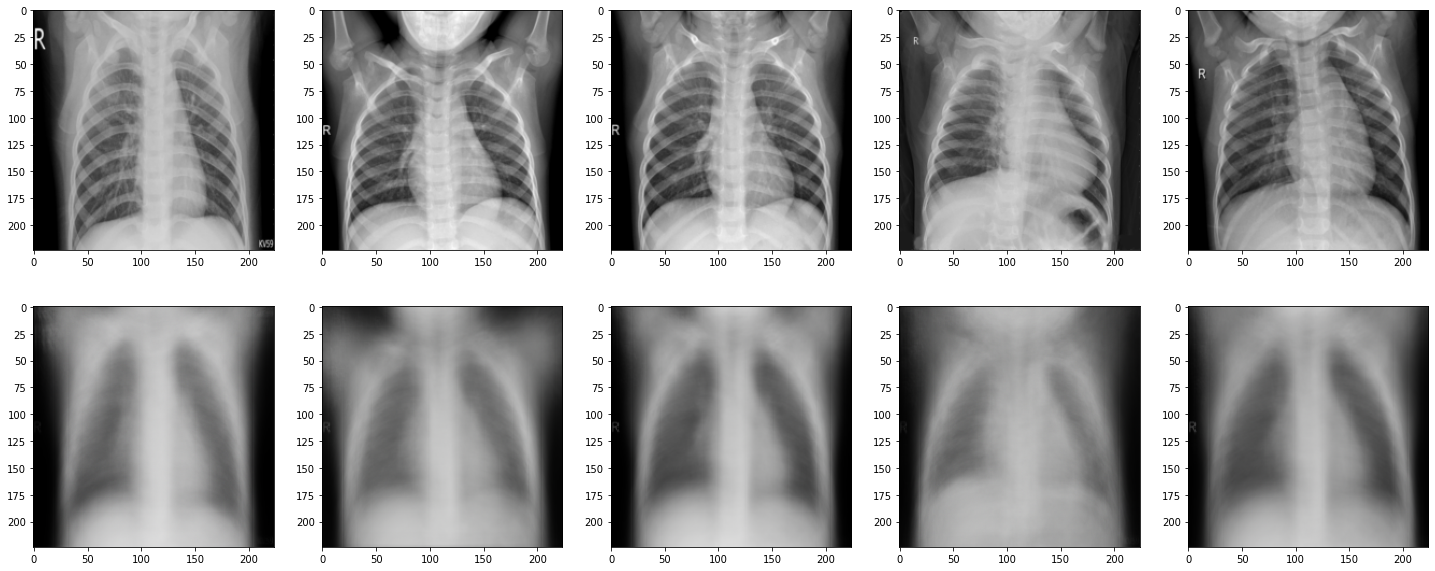
\includegraphics[width=0.7\textwidth]{./images/"contoh dataset"/Normal}
		\end{figure}
		\begin{figure}[h]
			\centering
			\caption{Gambar Chest X-Ray Pneumonia (atas) dengan Rekonstruksi (bawah).}
			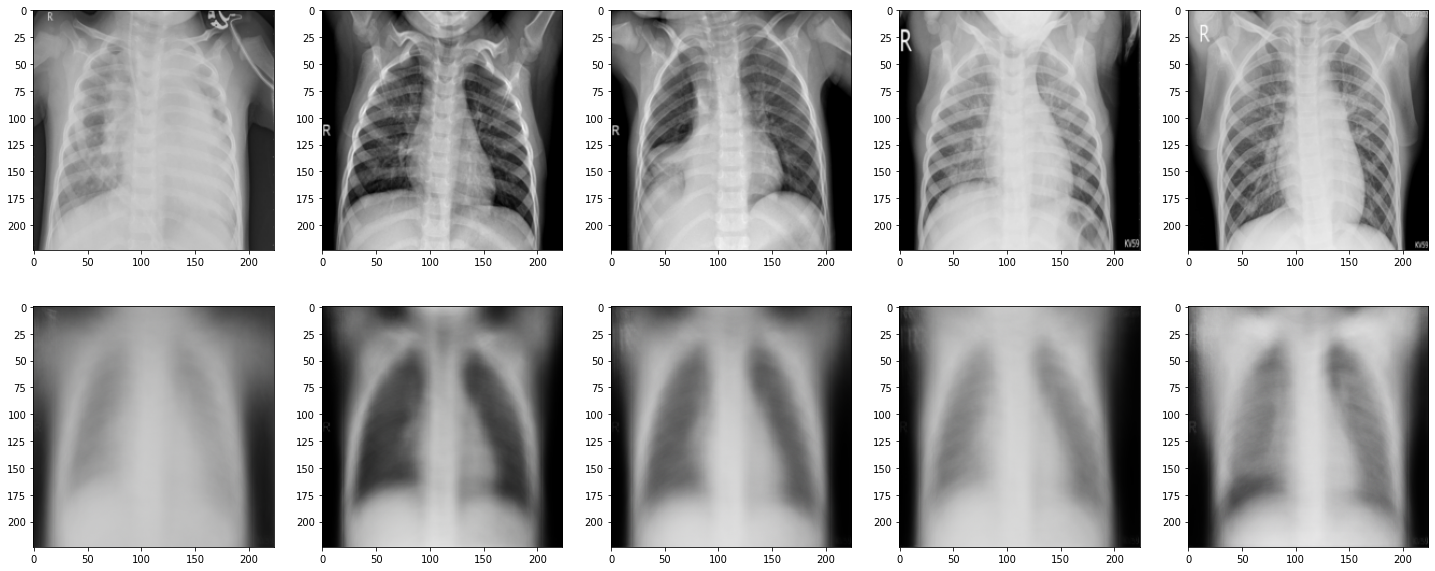
\includegraphics[width=0.7\textwidth]{./images/"contoh dataset"/Pneu}
		\end{figure}
		\begin{figure}[h]
			\centering
			\caption{Gambar Chest X-Ray COVID-19 (atas) dengan Rekonstruksi (bawah).}
			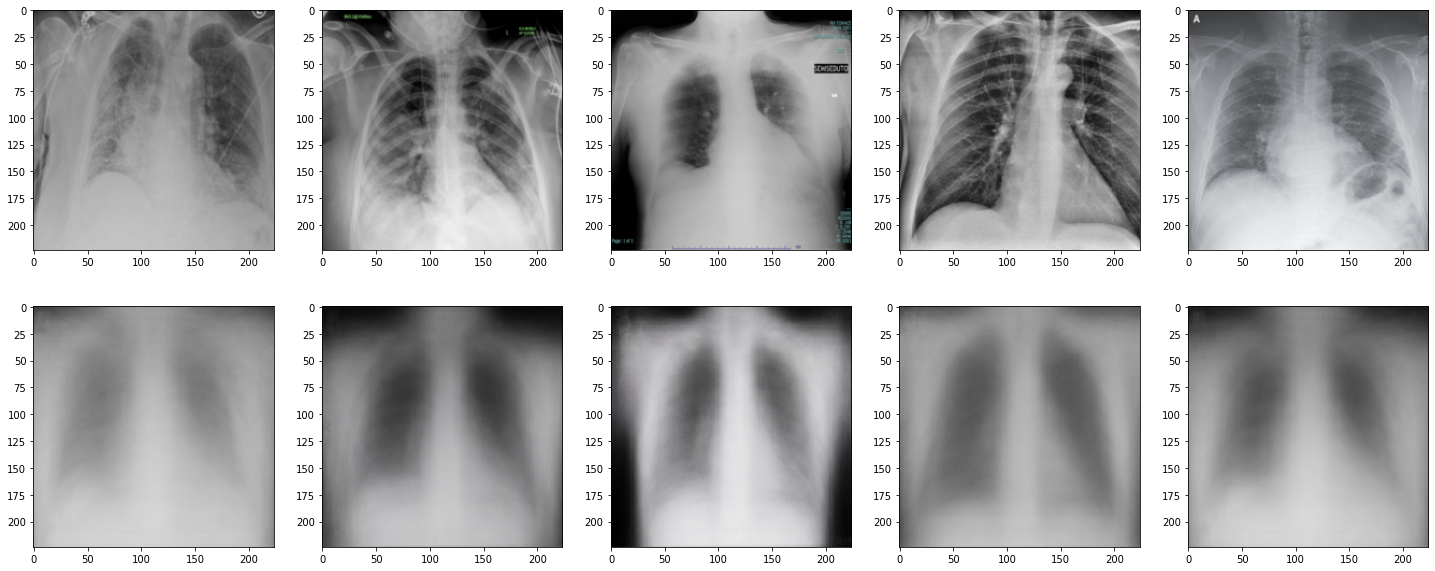
\includegraphics[width=0.7\textwidth]{./images/"contoh dataset"/Cov}
		\end{figure}
		\par
		Dari hasil rekonstruksi gambar pada figur diatas, walaupun input gambar memiliki perbedaan seperti lebih besar, memiliki kemiringan atau transformasi affine lain. Hasil rekonstruksi akhir model dapat tetap menjaga struktur fitur input gambar awal. Hasil rekonstruksi secara samar memiliki bentuk, struktur dan fitur-fitur yang menyerupai input gambar awal.
\end{document}